% \def\deso{0}
\begin{name}
	{\tenchude}
	{\tendethi}
	{\tentruong}
	{\thoigian}
\end{name}
%%%%Phần thầy Hoàng Thanh Phương
\TN
\Opensolutionfile{ans}[ans/2-TN-2025-PT2-TN]
\begin{ex}%[PT đề 2025, đề số 2]%[Hoàng Thanh Phương]%[2D4N1-2]
	Trên khoảng $(-\infty;-2)$, họ nguyên hàm của hàm số $f(x)=\dfrac{1}{x+2}$ là
	\choice
	{$\dfrac{1}{x+2}+C$}
	{\True $\ln |x+2|+C$}
	{$\dfrac{-1}{(x+2)^2}+C$}
	{$\dfrac{1}{2}\ln |x+2|$}
	\loigiai{
		Ta có $\displaystyle\int \dfrac{1}{x+2}\mathrm{\,d}x=\ln \left|x+2\right|+C$.
	}
\end{ex}
\begin{ex}%[PT đề 2025, đề số 2]%[Hoàng Thanh Phương]%[1D2N3-2]
	Cho cấp số nhân $(u_n)$ với $u_1=8$ và $u_2=4$. Công bội của cấp số nhân đã cho bằng
	\choice
	{\True $\dfrac{1}{2}$}
	{$-\dfrac{1}{2}$}
	{$-2$}
	{$2$}
	\loigiai{
		Ta có $u_2=u_1\cdot q\Leftrightarrow 4=8q\Leftrightarrow q=\dfrac{1}{2}$.
	}
\end{ex}
\begin{ex}%[PT đề 2025, đề số 2]%[Hoàng Thanh Phương]%[2H5N3-3]
	Trong không gian với hệ trục tọa độ $Oxyz$, mặt cầu tâm $I(1;0;0)$ và bán kính bằng $2$ có phương trình là
	\choice
	{$(x-1)^2+y^2+z^2=2$}
	{$(x+1)^2+y^2+z^2=2$}
	{\True $(x-1)^2+y^2+z^2=4$}
	{$(x+1)^2+y^2+z^2=4$}
	\loigiai{
		Phương trình mặt cầu cần tìm là $(x-1)^2+y^2+z^2=4$.
	}
\end{ex}
\begin{ex}%[PT đề 2025, đề số 2]%[Hoàng Thanh Phương]%[1H8H6-1]
	Cho hình chóp $S.ABC$ có đáy là tam giác vuông tại $B$, $AB=3a$, $BC=a\sqrt{3}$, $SA\perp (ABC)$ và $SA=2a$. Góc giữa đường thẳng $SC$ và mặt đáy $(ABC)$ bằng
	\choice
	{$60^\circ$}
	{$45^\circ$}
	{\True $30^\circ$}
	{$90^\circ$}
	\loigiai{
		\immini{
			Ta có $SA\perp (ABC)$ nên góc giữa $SC$ và $(ABC)$ là $\widehat{SCA}$. \\
			Xét tam giác $ABC$ vuông tại $B$ có 
			$$AC=\sqrt{AB^2+BC^2}=2a\sqrt{3}.$$
			Xét tam giác $SAC$ vuông tại $A$ có 
			$$\tan \widehat{SCA}=\dfrac{SA}{AC}=\dfrac{2a}{2a\sqrt{3}}=\dfrac{1}{\sqrt{3}},$$
			suy ra $\widehat{SCA}=30^\circ$.
		}
		{
			\begin{tikzpicture}[scale=0.8,>=stealth, font=\footnotesize, line join=round, line cap=round]
				\path 
				(0,0) coordinate (A)
				(1.5,-2) coordinate (B)
				(4.5,0) coordinate (C)
				($(A)+(0,4)$) coordinate (S)
				;
				\draw (S)--(A)--(B)--(S)--(C)--(B);
				\draw[dashed] (A)--(C);
				\foreach \d/\g in{A/180,B/-90,C/0,S/90}
				\draw[fill=black](\d)circle(1pt)node[shift={(\g:0.35)}]{$\d$};
				\foreach \x/\y/\z in {A/B/C}{
					\path pic[draw,angle radius=5pt]{right angle= \x--\y--\z};}
			\end{tikzpicture}	
		}
	}
\end{ex}
\begin{ex}%[PT đề 2025, đề số 2]%[Hoàng Thanh Phương]%[2D1N4-1]
	Cho hàm số $y=f(x)$ có bảng biến thiên như hình dưới đây. Số tiệm cận đứng và tiệm cận ngang của đồ thị hàm số đã cho là
	\begin{center}
		
\begin{tikzpicture}
			\tikzset{double style/.append style={double distance=1.5pt}}
			\tkzTabInit[nocadre=false,lgt=1.2,espcl=2.5,deltacl=0.6]
			{$x$ /0.6,$y'$ /0.6,$y$ /2}
			{$-\infty$,$-1$,$2$,$+\infty$}
			\tkzTabLine{,+,$0$,-,d,+,}
			\tkzTabVar{-/$-\infty$,+/$3$,-D-/$-\infty$/$-\infty$,+/$1$}
		\end{tikzpicture}
	\end{center}
	\choice
	{$0$}
	{\True $2$}
	{$1$}
	{$3$}
	\loigiai{
		Dựa vào bảng biến thiên, ta thấy $\lim\limits_{x\to2^+}y=-\infty$ và $\lim\limits_{x\to+\infty}y=1$ nên đồ thị hàm số đã cho có một đường tiệm cận đứng $x=2$ và một đường tiệm cận ngang $y=1$. \\
		Vậy đồ thị hàm số đã cho có $2$ đường tiệm cận đứng và tiệm cận ngang.
	}
\end{ex}
\begin{ex}%[PT đề 2025, đề số 2]%[Hoàng Thanh Phương]%[2D3H2-2]
	Khảo sát thời gian tập thể dục trong ngày của học sinh lớp $12$A và $12$B khối $12$ thu được mẫu số liệu ghép nhóm sau
	\begin{center}
		\begin{tabular}{|c|c|c|c|c|c|}
			\hline
			Thời gian (phút)& $[10;20)$ & $[20;30)$ & $[30;40)$& $[40;50)$ &$[50;60)$  \\
			\hline
			Số học sinh 12A& 5 & 7 & 12 & 10 &6  \\
			\hline
			Số học sinh 12B& 5 & 5 & 10 & 8 &12 \\
			\hline
		\end{tabular}
	\end{center}
	Gọi $s_1$ và $s_2$ lần lượt là độ lệch chuẩn của mẫu số liệu học sinh lớp $12A$ và $12B$. Hãy chọn phương án đúng?
	\choice
	{$s_1>s_2$}
	{\True $s_1<s_2$}
	{$s_1=s_2$}
	{$s_1>s_2^2$}
	\loigiai{
		Ta lập bảng có giá trị đại diện:
		\begin{center}
			\begin{tabular}{|c|c|c|c|c|c|c|}
				\hline
				Thời gian (phút)& $[10;20)$ & $[20;30)$ & $[30;40)$& $[40;50)$ &$[50;60)$  & \\
				\hline
				Giá trị đại diện &$15$ &$25$ &$35$ & $45$ & $55$ & \\
				\hline
				Số học sinh 12A& 5 & 7 & 12 & 10 &6 & $n=40$\\
				\hline
				Số học sinh 12B& 5 & 5 & 10 & 8 &12 & $n=40$\\
				\hline
			\end{tabular}
		\end{center}
		Xét học sinh lớp $12A$, ta có thời gian tập thể dục trung bình của lớp $12A$ là $\overline{x_A}=36{,}25$. \\
		Phương sai của mẫu số liệu của lớp $12A$ là
		\begin{eqnarray*}
			s_1^2&=&\dfrac{1}{40}\cdot \left[5(15-36{,}25)^2+7(25-36{,}25)^2+12(35-36{,}25)^2+10(45-36{,}25)^2+6(55-36{,}25)^2\right] \\
			&=&150{,}9375.
		\end{eqnarray*}
		Xét học sinh lớp $12B$, ta có thời gian tập thể dục trung bình của lớp $12B$ là $\overline{x_B}=39{,}25$. \\
		Phương sai của mẫu số liệu của lớp $12B$ là
		\begin{eqnarray*}
			s_2^2&=&\dfrac{1}{40}\cdot \left[5(15-39{,}25)^2+5(25-39{,}25)^2+10(35-39{,}25)^2+8(45-39{,}25)^2+12(55-39{,}25)^2\right] \\
			&=&184{,}4375.
		\end{eqnarray*}
		Ta có phương sai mẫu số liệu lớp $12B$ lớn hơn lớp $12A$, vậy độ lệch chuẩn của mẫu số liệu lớp $12B$ lớn hơn lớp $12A$.
	}
\end{ex}
\begin{ex}%[PT đề 2025, đề số 2]%[Hoàng Thanh Phương]%[1D6N4-3]
	Tập nghiệm của bất phương trình $2^x\le 4$ là
	\choice
	{\True $(-\infty;2]$}
	{$[0;2]$}
	{$(-\infty;2)$}
	{$(0;2)$}
	\loigiai{
		Ta có $2^x\le 4\Leftrightarrow x\le 2$ nên tập nghiệm của bất phương trình đã cho là $(-\infty;2]$.
	}
\end{ex}
\begin{ex}%[PT đề 2025, đề số 2]%[Hoàng Thanh Phương]%[2D4N3-1]
	\immini{Cho đồ thị hàm số $y=f(x)$ được xác định như hình vẽ. Diện tích $S$ của hình phẳng (phần gạch chéo) được xác định bởi 
		\choice
		{$S=\displaystyle\int\limits_{-2}^{2} f(x)\mathrm{\,d}x$}
		{$S=\displaystyle\int\limits_{-2}^{1} f(x)\mathrm{\,d}x+\displaystyle\int\limits_{1}^{2} f(x)\mathrm{\,d}x$}
		{\True $S=-\displaystyle\int\limits_{-2}^{1} f(x)\mathrm{\,d}x+\displaystyle\int\limits_{1}^{2} f(x)\mathrm{\,d}x$}
		{$S=\displaystyle\int\limits_{-2}^{1} f(x)\mathrm{\,d}x-\displaystyle\int\limits_{1}^{2} f(x)\mathrm{\,d}x$}}
	{
		\begin{tikzpicture}[scale=0.8,>=stealth, font=\footnotesize, line join=round, line cap=round]
			\def\xmin{-3} \def\xmax{3}
			\def\ymin{-4} \def\ymax{3}  (\xmin,\ymin) grid (\xmax,\ymax); 
			\draw[->] (\xmin,0)--(\xmax,0) node [below]{$x$};
			\draw[->] (0,\ymin)--(0,\ymax) node [left]{$y$};
			\node at (0,0) [below left]{$O$};
			\clip (\xmin+0.1,\ymin+0.1) rectangle (\xmax-0.1,\ymax-0.1);
			\draw[smooth,samples=300,domain=-2.5:3] plot(\x,{-0.5*(\x+2)*(\x-1)*(\x-2)});
			\fill[pattern=north east lines,opacity=0.7] plot[domain=-2:2](\x,{-0.5*(\x+2)*(\x-1)*(\x-2)});
			\foreach \d/\g in{-2/-135,1/-90,2/-120}
			\draw[fill=black](\d,0)circle(1pt)node[shift={(\g:0.35)}]{$\d$};
		\end{tikzpicture}
	}
	\loigiai{
		Dựa vào hình vẽ, ta thấy $S=-\displaystyle\int\limits_{-2}^{1} f(x)\mathrm{\,d}x+\displaystyle\int\limits_{1}^{2} f(x)\mathrm{\,d}x$.
	}
\end{ex}
\begin{ex}%[PT đề 2025, đề số 2]%[Hoàng Thanh Phương]%[2D1H5-1]
	\immini{Hàm số nào dưới đây có đồ thị như hình vẽ?
		\choice
		{$y=\dfrac{x^2-2x+5}{x+2}$}
		{$y=\dfrac{x^2-2x}{x+2}$}
		{$y=\dfrac{x^2+4x+5}{x-2}$}
		{\True $y=\dfrac{x^2+4x+5}{x+2}$}}
	{
		\begin{tikzpicture}[scale=0.7,>=stealth, font=\footnotesize, line join=round, line cap=round]
			\def\a{1} \def\b{4} \def\c{5} \def\d{1} \def\e{2}% Hệ số
			\def\xmin{-5} \def\xmax{3}
			\def\ymin{-4} \def\ymax{4}
			\draw[->] (\xmin,0)--(\xmax,0) node [below]{$x$};
			\draw[->] (0,\ymin)--(0,\ymax) node [left]{$y$};
			\node at (0,0) [below left]{$O$};
			\clip (\xmin+0.1,\ymin+0.1) rectangle (\xmax-0.1,\ymax-0.1);
			\draw[smooth,samples=300,domain=\xmin:(-\e/\d-0.1)] plot(\x,{(\a*(\x)^2+\b*(\x)+\c)/(\d*(\x)+\e)});
			\draw[smooth,samples=300,domain=(-\e/\d+0.1:\xmax)] plot(\x,{(\a*(\x)^2+\b*(\x)+\c)/(\d*(\x)+\e)});
			\draw[dashed] (-\e/\d,\ymin)--(-\e/\d,\ymax);
			\draw[smooth,thin,samples=300,domain=\xmin:\xmax] plot(\x,{(\a*(\x)/(\d)+(\d*\b-\e*\a)/((\d)^2)});
			\draw[dashed] (-3,0)--(-3,-2)--(0,-2) (-1,0)--(-1,2)--(0,2);
			\foreach \d/\g in{-3/90,-2/-60,-1/-90}
			\draw[fill=black](\d,0)circle(1pt)node[shift={(\g:0.35)}]{$\d$};
			\foreach \d/\g in{-2/0,2/0}
			\draw[fill=black](0,\d)circle(1pt)node[shift={(\g:0.35)}]{$\d$};
		\end{tikzpicture}
	}
	\loigiai{
		Dựa vào đồ thị, ta thấy đồ thị hàm số có tiệm cận đứng $x=-2$ và tiệm cận xiên $y=x+2$. 
		\begin{itemize}
			\item Xét hàm số $y=\dfrac{x^2-2x+5}{x+2}$, đồ thị hàm số này có tiệm cận xiên $y=x-4$ nên không thỏa mãn.
			\item Xét hàm số $y=\dfrac{x^2-2x}{x+2}$, đồ thị hàm số này có tiệm cận xiên $y=x-4$ nên không thỏa mãn.
			\item Xét hàm số $y=\dfrac{x^2+4x+5}{x-2}$, đồ thị hàm số này có tiệm cận đứng $x=2$ nên không thỏa mãn.
			\item Xét hàm số $y=\dfrac{x^2+4x+5}{x+2}$, đồ thị này có tiệm cận đứng $x=-2$ và tiệm cận xiên $y=x+2$ nên thỏa mãn yêu cầu bài toán. 
		\end{itemize}
		Vậy hàm số cần tìm là $y=\dfrac{x^2+4x+5}{x+2}$.
	}
\end{ex}
\begin{ex}%[PT đề 2025, đề số 2]%[Hoàng Thanh Phương]%[2H2H1-2]
	Cho tứ diện $ABCD$. Đặt $\vec{AB} =a$, $\vec{AC}=b$ và $\vec{AD}=c$. Gọi $G$ là trọng tâm tam giác $BCD$. Mệnh đề nào sau đây đúng?
	\choice
	{$\vec{AG}=\vec{a}+\vec{b}+\vec{c}$}
	{$\vec{AG}=\dfrac{1}{2}\left(\vec{a}+\vec{b}+\vec{c}\right)$}
	{\True $\vec{AG}=\dfrac{1}{3}\left(\vec{a}+\vec{b}+\vec{c}\right)$}
	{$\vec{AG}=\dfrac{1}{4}\left(\vec{a}+\vec{b}+\vec{c}\right)$}
	\loigiai{
		\immini{
			Xét tam giác $BCD$ với trọng tâm $G$. Áp dụng quy tắc trọng tâm, ta có 
			$$\vec{MB}+\vec{MC}+\vec{MD}=3\vec{MG},$$
			với điểm $M$ tùy ý. \\
			Lấy $M\equiv A$, ta có $\vec{AB}+\vec{AC}+\vec{AD}=3\vec{AG}$. \\
			Vậy $\vec{AG}=\dfrac{1}{3}\left(\vec{AB}+\vec{AC}+\vec{AD}\right)=\dfrac{1}{3}\left(\vec{a}+\vec{b}+\vec{c}\right)$.
		}
		{
			\begin{tikzpicture}[scale=0.8,>=stealth, font=\footnotesize, line join=round, line cap=round]
				\path 
				(0,0) coordinate (B)
				(1.5,-2) coordinate (C)
				(4.5,0) coordinate (D)
				($(B)+(1,4)$) coordinate (A)
				($(C)!0.5!(D)$) coordinate (M)
				($(B)!2/3!(M)$) coordinate (G)
				;
				\draw (A)--(B)--(C)--(A)--(D)--(C);
				\draw[dashed] (A)--(G)--(B) (C)--(G)--(D)--(B);
				\foreach \d/\g in{A/90,B/180,C/-90,D/0,G/-45}
				\draw[fill=black](\d)circle(1pt)node[shift={(\g:0.35)}]{$\d$};
			\end{tikzpicture}	
			
		}
		
	}
\end{ex}
\begin{ex}%[PT đề 2025, đề số 2]%[Hoàng Thanh Phương]%[2D4N2-2]
	Nếu $\displaystyle\int\limits_{0}^{1} \left[f(x)+2x\right]\mathrm{\,d}x=3$ thì $\displaystyle\int\limits_{0}^{1} f(x)\mathrm{\,d}x$ bằng
	\choice
	{$3$}
	{$1$}
	{\True $2$}
	{$0$}
	\loigiai{
		Ta có $$\displaystyle\int\limits_{0}^{1} \left[f(x)+2x\right]\mathrm{\,d}x=\displaystyle\int\limits_{0}^{1} f(x)\mathrm{\,d}x+\displaystyle\int\limits_{0}^{1} 2x\mathrm{\,d}x\Leftrightarrow 3=\displaystyle\int\limits_{0}^{1} f(x)\mathrm{\,d}x+1\Leftrightarrow \displaystyle\int\limits_{0}^{1} f(x)\mathrm{\,d}x=2.$$
	}
\end{ex}
\begin{ex}%[PT đề 2025, đề số 2]%[Hoàng Thanh Phương]%[1D6N4-2]
	Nghiệm của phương trình $\log (4x-6)=1$ là
	\choice
	{$x=\dfrac{9}{2}$}
	{$x=\dfrac{7}{4}$}
	{\True $x=4$}
	{$x=5$}
	\loigiai{
		Ta có $\log (4x-6)=1\Leftrightarrow 4x-6=10\Leftrightarrow x=4$.
	}
\end{ex}
%%%%Phần thầy Trần Hưng
\Closesolutionfile{ans}
% \indapan{6}{ans/2-TN-2025-PT2-TN}
\cauds
\Opensolutionfile{ans}[ans/2-TN-2025-PT2-DS]
\begin{ex}%[PT đề 2025, đề số 2]%[Trần Văn Hưng]%[2D1H4-1]
	Cho hàm số $f(x)=\dfrac{x^2-4x+5}{x-1}$.
	\choiceTF
	{\True Hàm số có đạo hàm $f'(x)=\dfrac{x^2-2x-1}{(x-1)^2}$}	
	{Hàm số đồng biến trên khoảng $(-\infty;1)$}	
	{\True Hàm số đạt cực tiểu tại $x=1+\sqrt{2}$}
	{\True Đường thẳng $y=x-3$ là tiệm cận xiên của đồ thị hàm số}
	\loigiai{
		Hàm số $f(x)$ có tập xác định $\mathscr{D}=\mathbb{R}\setminus\{1\}$.
		\begin{itemchoice}
			\itemch Ta có
			\[f'(x) = \dfrac{(2x - 4)\cdot(x - 1) - (x^2 - 4x + 5)\cdot 1}{(x - 1)^2}	
			= \dfrac{x^2 - 2x -1}{(x - 1)^2}.\]	
			\itemch Ta có $f'(x)=0\Leftrightarrow x^2-2x-1=0\Leftrightarrow x=1\pm \sqrt{2}$.\\
			Bảng biến thiên
			\begin{center}
				
\begin{tikzpicture}
					\tkzTabInit[nocadre=false,lgt=1.2,espcl=2.5,deltacl=0.6]
					{$x$ /0.6,$f'(x)$ /0.6, $f(x)$/2.5}
					{$-\infty$,$1-\sqrt{2}$,$1$,$1+\sqrt{2}$,$+\infty$}
					\tkzTabLine{,+,$0$,-,d,-,$0$,+,}
					\tkzTabVar{-/$-\infty$,+/$-2-2\sqrt{2}$,-D+/$-\infty$/$+\infty$,-/$-2+2\sqrt{2}$,+/$+\infty$}
				\end{tikzpicture}
			\end{center}
			Từ bảng biến thiên suy ra hàm số đồng biến trên các khoảng $\left(-\infty;1-\sqrt{2}\right)$ và $\left(1+\sqrt{2};+\infty\right)$.
			\itemch Từ bảng biến thiên suy ra hàm số đạt cực tiểu tại điểm $x=1+\sqrt{2}$.
			\itemch Ta có\\
			$\lim\limits_{x\to -\infty}\left[\dfrac{x^2-4x+5}{x-1}-(x-3)\right]=\lim\limits_{x\to -\infty}\dfrac{2}{x-1}=0$.\\
			$\lim\limits_{x\to +\infty}\left[\dfrac{x^2-4x+5}{x-1}-(x-3)\right]=\lim\limits_{x\to +\infty}\dfrac{2}{x-1}=0$.\\
			Do đó $y=x-3$ là tiệm cận xiên của đồ thị hàm số.
		\end{itemchoice}
	}
\end{ex}
\begin{ex}%[PT đề 2025, đề số 2]%[Trần Văn Hưng]%[2D4V1-6]
	Một công ty ước tính doanh thu biên là $R'(q)=278-2q$ (USD) khi bán hết $q$ sản phẩm. Chi phí biên tương ứng để sản xuất $q$ sản phẩm là $C'(q)=1{,}2q^2-2q+8$ (USD). Giả sử khi công ty sản xuất và bán được $5$ sản phẩm thì lợi nhuận của công ty là $1\,210$ USD. 
	(Với $R(q)$ là hàm doanh thu khi bán hết $q$ sản phẩm, $C(q)$ là hàm chi phí để sản xuất $q$ sản phẩm, $P(q)$ là hàm lợi nhuận khi sản xuất và bán hết $q$ sản phẩm). 
	\choiceTF
	{\True Lợi nhuận của công ty tại khi bán sản xuất và bán hết $q$ sản phẩm là $P(q)=R(q)-C(q)$}
	{$P(q)=-0{,}4q^3+270q+90$}
	{\True Công ty đạt lợi nhuận tối đa khi sản xuất và bán hết $15$ sản phẩm}
	{Lợi nhuận của công ty khi sản xuất và bán hết $25$ sản phẩm là $590$ USD}
	\loigiai{
		\begin{itemchoice}
			\itemch Lợi nhuận của công ty tại sản phẩm thứ $q$ bằng tổng doanh thu trừ đi tổng chi phí khi công ty sản xuất ra $q$ sản phẩm.
			Do đó, $P(q)=R(q)-C(q)$.
			\itemch Ta có 
			\begin{eqnarray*}
				P(q)&=&R(q)-C(q)\\
				&=&\displaystyle\int R'(q)\mathrm{\,d}q-\displaystyle\int C'(q) \mathrm{\,d}q\\
				&=&\displaystyle\int (278-2q)\mathrm{\,d}q-\displaystyle\int (1{,}2q^2-2q+8)\mathrm{\,d}q\\
				&=&-0{,}4q^3+270q+C.
			\end{eqnarray*}			
			Lợi nhuận của công ty là $1210$ USD nên $P(5)=1\,210$.\\
			Khi đó, ta có $-0{,}4\cdot5^3+270\cdot5+C=1\,210\Rightarrow C=-90$.\\
			Do đó, $P(q)=-0{,}4q^3+270q-90$ (USD).
			\itemch $P'(q)=-1{,}2q^2+270=0\Leftrightarrow q=15$ $(q=-15<0$, loại).\\
			Bảng biến thiên của hàm số $P(q)$ như sau
			\begin{center}
				
\begin{tikzpicture}
					\tkzTabInit[nocadre=false,lgt=1.2,espcl=3,deltacl=0.6]
					{$q$/0.7,$P'(q)$/0.7,$P(q)$/2}{$0$,$15$,$+\infty$}
					\tkzTabLine{,+,0,-,}   
					\tkzTabVar{-/$-90$,+/$2\,610$,-/$-\infty$}
				\end{tikzpicture}
			\end{center}
			Từ bảng biến thiên, ta thấy công ty đạt lợi nhuận công ty tối đa khi sản xuất và bán được $15$ sản phẩm.
			\itemch Ta có $P(25)=-0{,}4\cdot25^3+270\cdot25-90=410$ (USD).
	\end{itemchoice}}
\end{ex}
%%%% Phần thầy Nguyễn Trung Kiên
\begin{ex}%[Đề phát triển 02]%[Nguyễn Trung Kiên, dự án TeX hóa và phát triển đề tốt nghiệp năm 2025]%[2H5V2-3]
	Trong một quan sát chuyển động của một vật, người ta mô hình bằng cách chọn một hệ trục tọa độ $Oxyz$ trong không gian với các vectơ $\overrightarrow{i}$, $\overrightarrow{j}$, $\overrightarrow{k}$ lần lượt là các vectơ đơn vị của các trục $Ox$, $Oy$, $Oz$ và độ dài của các vectơ đơn vị đó là mét. Vật được quan sát coi như một chất điểm, ban đầu vật ở vị trí $A(100;120;0)$ được phóng đi theo đường thẳng $\Delta$ với hướng phóng là vectơ $\overrightarrow{u}=(a;b;c)$, vận tốc phóng $v(t)=kt$ (m/s), thời gian $t$ tính bằng giây và $0\leq t\leq 10$. Biết rằng vectơ $\overrightarrow{u}$ có độ dài bằng $2$ và tạo với các vectơ $\overrightarrow{i}$, $\overrightarrow{j}$, $\overrightarrow{k}$ các góc lần lượt là $120^\circ$, $60^\circ$, $45^\circ$. Tại thời điểm $2$ giây sau khi phóng vật đạt độ cao $80\sqrt{2}$ mét so với vị trí ban đầu. 
	\choiceTF
	{$\overrightarrow{u} \cdot \overrightarrow{i}= \cos{120^\circ}$}
	{\True Phương trình đường thẳng $\Delta$ là $\dfrac{x-100}{-1}=\dfrac{y-120}{1}=\dfrac{z}{\sqrt{2}}$}
	{\True Vận tốc của vật tại thời điểm $t=5$ giây sau khi phóng là $400$ m/s}
	{\True Giả sử tại $M(20;800;20)$ có một trạm quan sát, sau $8$ giây kể từ khi phóng khoảng cách từ trạm quan sát $M$ đến vật lớn hơn $2\,200$ mét}
	\loigiai
	{Vì $\overrightarrow{i}$, $\overrightarrow{j}$, $\overrightarrow{k}$ lần lượt là vectơ đơn vị của các trục $Ox$, $Oy$, $Oz$ nên $\overrightarrow{i}=(1;0;0)$, $\overrightarrow{j}=(0;1;0)$ và $\overrightarrow{k}=(0;0;1)$.
		\begin{itemchoice}
			\itemch Ta có $\overrightarrow{u} \cdot \overrightarrow{i} = \left|\overrightarrow{u}\right| \cdot \left|\overrightarrow{i}\right| \cdot \cos\left(\overrightarrow{u}, \overrightarrow{i}\right) = 2 \cdot 1 \cdot \cos{120^\circ} = 2\cos{120^\circ}$.
			\itemch Vì $\overrightarrow{u} \cdot \overrightarrow{i} = \left|\overrightarrow{u}\right| \cdot \left|\overrightarrow{i}\right| \cdot \cos\left(\overrightarrow{u}, \overrightarrow{i}\right) \Leftrightarrow a+0+0=2\cos{120^\circ} \Leftrightarrow a=-1$.\\
			Tương tự, $\overrightarrow{u} \cdot \overrightarrow{j} = \left|\overrightarrow{u}\right| \cdot \left|\overrightarrow{j}\right| \cdot \cos\left(\overrightarrow{u}, \overrightarrow{j}\right) \Leftrightarrow 0+b+0=2\cos{60^\circ} \Leftrightarrow b=1$.\\
			Tương tự, $\overrightarrow{u} \cdot \overrightarrow{k} = \left|\overrightarrow{u}\right| \cdot \left|\overrightarrow{k}\right| \cdot \cos\left(\overrightarrow{u}, \overrightarrow{k}\right) \Leftrightarrow 0+0+c=2\cos{45^\circ} \Leftrightarrow c=\sqrt{2}$.\\
			Suy ra, $\overrightarrow{u}=\left(-1;1;\sqrt{2}\right)$.\\
			Đường thẳng $\Delta$ đi qua điểm $A$ và nhận vectơ $\overrightarrow{u}$ làm vectơ chỉ phương nên có phương trình
			$$\dfrac{x-100}{-1} = \dfrac{y-120}{1} = \dfrac{z}{\sqrt{2}}.$$
			\itemch Giả sử tại thời điểm $2$ giây sau khi phóng, vật ở vị trí $B$, khi đó $B\left(100-b; 120+b;b\sqrt{2}\right)$.\\
			Do vật đạt độ cao $80\sqrt{2}$ mét so với vị trí điểm $A$ nên $z_B-z_A=80\sqrt{2} \Leftrightarrow b=80 \Rightarrow B\left(20;200;80\sqrt{2}\right)$.\\
			Quãng đường vật đi được là $AB=\sqrt{(-80)^2+80^2+\left(80\sqrt{2}\right)^2} = 160$ (m).\\
			Do đó $\displaystyle\int\limits_{0}^{2} v(t) \mathrm{\,d}t = 160 \Leftrightarrow \displaystyle\int\limits_{0}^{2} kt \mathrm{\,d}t = 160 \Leftrightarrow \dfrac{kt^2}{2} \Bigg|_0^2 = 160 \Leftrightarrow 2k=160 \Leftrightarrow k=80$.\\
			Vậy $v(t)=80t$ (m/s) với $0\leq t\leq 10$ và $v(5)=400$ (m/s).
			\itemch Giả sử sau $8$ giây kể từ khi được phóng đi, vật ở vị trí $C$, khi đó $\overrightarrow{AC}$ cùng hướng với $\overrightarrow{u}$ nên $\overrightarrow{AC}=c\overrightarrow{u}$ ($c>0$), do đó $C(100-c;120+c;c\sqrt{2})$ và $AC=\sqrt{(-c)^2+c^2+\left(c\sqrt{2}\right)^2}=2c$.\\
			Mặt khác
			$$AC=\displaystyle\int\limits_{0}^{8} v(t) \mathrm{\,d}t \Leftrightarrow 2c = \displaystyle\int\limits_{0}^{8} 80t \mathrm{\,d}t \Leftrightarrow c = 1280 \Rightarrow C\left(-1\,180; 1\,400; 1\,280\sqrt{2}\right).$$
			Khoảng cách từ trạm quan sát đến vật là $$MC = \sqrt{(-1\,200)^2+600^2+\left(1\,280\sqrt{2}-20\right)^2} \approx 2\,237 \text{  (mét)}.$$
		\end{itemchoice}
	}
\end{ex}
\begin{ex}%[Đề phát triển 02]%[Nguyễn Trung Kiên, dự án TeX hóa và phát triển đề tốt nghiệp năm 2025]%[2D6V2-4]
	Một nhà máy có ba phân xưởng sản xuất cùng thực hiện sản xuất một sản phẩm. Phân xưởng I sản xuất $40\%$ trong tổng số lượng sản phẩm của nhà máy và tỉ lệ sản phẩm bị lỗi của phân xưởng I là $5\%$. Phân xưởng II sản xuất $32\%$ trong tổng số lượng sản phẩm của nhà máy và tỉ lệ sản phẩm bị lỗi của phân xưởng II là $6\%$. Trong quá trình kiểm tra người ta lấy ngẫu nhiên một sản phẩm trong số sản phẩm do hai phân xưởng I và II sản xuất.
	\choiceTF
	{Xác suất để sản phẩm lấy được của phân xưởng I là $0{,}4$}
	{\True Xác suất để sản phẩm lấy được không bị lỗi và của phân xưởng II là $\dfrac{94}{225}$}
	{\True Xác suất để sản phẩm lấy được bị lỗi là $\dfrac{49}{900}$}
	{Biết rằng sản phẩm lấy ra bị lỗi, xác suất sản phẩm đó của phân xưởng I là $0{,}45$}
	\loigiai
	{Gọi $A$ là biến cố \lq\lq Sản phẩm lấy được của phân xưởng I\rq\rq;\\
		$B$ là biến cố \lq\lq Sản phẩm lấy được là sản phẩm bị lỗi\rq\rq.\\
		Vì tổng số sản phẩm hai phân xưởng I và II sản xuất chiếm $40\%+32\% = 72\%$ số sản phẩm của nhà máy nên xác suất để sản phẩm lấy được của phân xưởng I là $\mathrm{P}(A)=\dfrac{40}{72} = \dfrac{5}{9}$.\\
		Từ đó ta có, xác suất để sản phẩm lấy được của phân xưởng II là $\mathrm{P}\left(\overline{A}\right)=1- \mathrm{P}(A) = \dfrac{4}{9}$.\\
		Mặt khác, theo bài ra ta có $\mathrm{P}(B\mid A) = 5\% = 0{,}05$ và $\mathrm{P}\left(B\mid \overline{A}\right)=6\% = 0{,}06$.\\
		Ta có sơ đồ cây như sau
		\begin{center}
			\begin{tikzpicture}[scale=1.2, font=\footnotesize, line join=round, line cap=round, >=stealth]
				\path (0,0) coordinate(O) 
				(2.5,1) node[draw, fill=red!10!white, rounded corners=1mm, outer sep=2pt](A1){$A$}
				(2.5,-1) node[draw, fill=red!10!white, rounded corners=1mm, outer sep=2pt](A2){$\overline{A}$}
				(5,1.5) node[draw, fill=blue!10!white, rounded corners=1mm, outer sep=2pt](B1){$B$}
				(5,0.5) node[draw, fill=blue!10!white, rounded corners=1mm, outer sep=2pt](B2){$\overline{B}$}
				(5,-0.5) node[draw, fill=blue!10!white, rounded corners=1mm, outer sep=2pt](B3){$B$}
				(5,-1.5) node[draw, fill=blue!10!white, rounded corners=1mm, outer sep=2pt](B4){$\overline{B}$};
				\fill (O) circle(1pt);
				\draw[->] (O)--(A1) node[midway, sloped, above]{$\dfrac{5}{9}$};
				\draw[->] (O)--(A2) node[midway, sloped, below]{$\dfrac{4}{9}$};
				\draw[->] (A1)--(B1) node[midway, sloped, above]{$0{,}05$};
				\draw[->] (A1)--(B2) node[midway, sloped, below]{$0{,}95$};
				\draw[->] (A2)--(B3) node[midway, sloped, above]{$0{,}06$};
				\draw[->] (A2)--(B4) node[midway, sloped, below]{$0{,}94$};
			\end{tikzpicture}
		\end{center}
		\begin{itemchoice}
			\itemch Xác suất để sản phẩm lấy được của phân xưởng I là $\mathrm{P}(A)=\dfrac{5}{9}$.
			\itemch Xác suất để sản phẩm lấy được không bị lỗi và của phân xưởng II là $$\mathrm{P}\left(\overline{B}\,\overline{A}\right) = \mathrm{P}\left(\overline{A}\right) \cdot \mathrm{P}\left(\overline{B} \mid \overline{A}\right) = \dfrac{4}{9} \cdot 0{,}94 = \dfrac{94}{225}.$$
			\itemch Xác suất để sản phẩm lấy được bị lỗi là 
			$$\mathrm{P}(B) = \mathrm{P}(A) \cdot \mathrm{P}(B\mid A) + \mathrm{P}\left(\overline{A}\right) \cdot \mathrm{P}\left(B\mid \overline{A}\right) = \dfrac{5}{9}\cdot 0{,}05 + \dfrac{4}{9}\cdot 0{,}06 = \dfrac{49}{900}.$$
			\itemch Biết rằng sản phẩm lấy ra bị lỗi, xác suất sản phẩm đó của phân xưởng I là
			$$\mathrm{P}\left(A\mid B\right)= \dfrac{\mathrm{P}(A)\cdot \mathrm{P}(B\mid A)}{\mathrm{P}(B)} = \dfrac{\dfrac{5}{9}\cdot 0{,}05}{\dfrac{49}{900}} = \dfrac{25}{49}.$$
		\end{itemchoice}
	}
\end{ex}
\Closesolutionfile{ans}
% \indapan{2}{ans/2-TN-2025-PT2-DS}
\caukq
\Opensolutionfile{ans}[ans/2-TN-2025-PT2-KQ]
%%%%Phần thầy Nam Nhất Trần
\begin{ex}%[Đề phát triển 02]%[Nam Nhất Trần, dự án TeX hóa và phát triển đề tốt nghiệp năm 2025]%[0D0C2-5]
	Xung quanh bờ hồ hình tròn, người ta trồng $10$ cây chuối. Người ta chặt ngẫu nhiên $4$ cây chuối. 
	Xác suất để $4$ cây bị chặt không có hai cây nào đứng cạnh nhau bằng $\dfrac{a}{b}$ tối giản, tính giá trị $a+b$?
	\shortans{47}
	\loigiai{
		\textbf{Cách 1.} \\
		Đánh số các cây trên bờ hồ hình tròn từ $1$ đến $10$. \\ 
		Đánh số 4 câu được chọn ngẫu nhiên là $a$, $b$, $c$, $d$ theo thứ tự tăng dần. \\
		Số phần tử không gian mẫu là $\mathrm{C}^4_{10}$. \\
		Gọi $A$ biến cố thỏa bài toán thì $A$: \lq\lq $1\leq a < b-1 < c-2 < d-3 \leq 7$ \rq\rq. 
		\begin{itemize}
			\item Trường hợp 1. $a=1$. Khi đó $\heva{&b\geq 3 \\&d\leq 9} \Rightarrow \heva{&b-1 \geq 2 \\&d-3 \leq 6.}$ \\
			Từ tập $\{2;3;4;5;6\}$, chọn $3$ số và xếp theo tứ tự tăng dần (vào $b-1$, $c-2$, $d-3$), có $\mathrm{C}^3_{5}$ cách. \\
			Mỗi cách chọn trên tương ứng với một cách chọn cho $b$, $c$, $d$ thỏa bài toán. \\
			Vậy trường hợp này có $\mathrm{C}^3_{5}$ cách.
			\item Trường hợp 2. $a\geq 2$. \\
			Từ tập $\{2;3;4;5;6;7\}$ chọn 4 số theo và xếp theo thứ tự tăng dần (vào $a$, $b-1$, $c-2$, $d-3$), có $\mathrm{C}^4_{6}$ cách.\\
			Mỗi cách chọn trên tương ứng với một cách chọn cho $a$, $b$, $c$, $d$ thỏa bài toán. \\
			Vậy trường hợp này có $\mathrm{C}^4_{6}$ cách.
		\end{itemize}
		Từ hai trường hợp trên suy ra $n(A)=\mathrm{C}^3_{5}+\mathrm{C}^4_{6}=25$ và xác suất của biến cố $A$ là $\mathrm{P}(A)=\dfrac{n(A)}{n(\Omega)}=\dfrac{5}{42}$.
		\\
		\textbf{Cách 2.} \\
		Ta nhắc lại bài toán chia kẹo Euler dạng cơ bản: Phương trình
		$$x_1+x_2+...+x_k=n$$
		với điều kiện $n\ge k$, có $\mathrm{C}^{k-1}_{n+k-1}$ nghiệm nguyên không âm.
		\begin{itemize}
			\item Trường hợp 1, giả sử chặt cây $1$. Khi đó cây $2$ và cây $10$ sẽ không bị chặt, vậy ba cây còn lại bị chặt là ba trong số các cây từ $3$ đến $9$. \\
			Gọi $x_1$, $x_2$, $x_3$, $x_4$ lần lượt là số lượng cây nằm ở giữa bốn cây bị chặt (chưa bao gồm cây $2$ và cây $10$). \\
			Vậy ta có $x_1+x_2+x_3+x_4=4$. Đồng thời $x_1\ge 0$, $x_2\ge 1$, $x_3\ge 1$ và $x_4\ge 0$ (do đã có cây $2$ và cây $10$ đứng cạnh cây $1$ bị chặt, nên $x_1$ và $x_4$ có thể bằng $0$ vẫn thỏa mãn yêu cầu đề bài). \\ 
			Đặt $x_2=y_2+1$, $x_3=y_3+1$, suy ra $x_1+y_2+y_3+x_4=2$ và $x_1,  y_2, y_3, x_4\ge 0$. \\
			Áp dụng bài toán chia kẹo Euler, ta có số cách chặt là $\mathrm{C}^3_5=10$ cách.
			\item Trường hợp $2$, giả sử cây bị chặt không phải cây $1$. \\
			Ta ``trải hình'' thành đường thẳng, duỗi đường tròn tại vị trí cây số $1$. Khi đó, ta xét các cây từ $2$ đến $10$. \\
			Ta gọi $x_1$, $x_2$, $x_3$, $x_4$, $x_5$ lần lượt là số cây chưa bị chặt nằm bên trái cây bị chặt số $1$, số cây nằm giữa cây bị chặt $1$ và $2$, số cây nằm giữa cây bị chặt $2$ và $3$, số cây nằm giữa cây bị chặt $3$ và $4$, số cây nằm bên phải cây bị chặt số $4$. \\
			Vậy ta có $x_1+x_2+x_3+x_4+x_5=5$ (do từ $2$ đến $10$ có $9$ cây, chặt mất $4$ cây nên còn $5$ cây). \\
			Ngoài ra, ta có $x_2, x_3, x_4\ge 1$, đồng thời $x_1\ge 0$ và $x_5\ge 0$. \\
			Đặt $x_2=y_2+1$, $x_3=y_3+1$, $x_4=y_4+1$, ta có $x_1+y_2+y_3+y_4+x_5=2$ và $x_1,y_2,y_3,y_4,x_5\ge 0$. \\
			Áp dụng bài toán chia kẹo Euler, ta có số cách chặt cây là $\mathrm{C}^4_6=15$ cách.
		\end{itemize}
		Vậy có $25$ cách chặt thỏa mãn yêu cầu, suy ra xác suất cần tính là $\dfrac{25}{\mathrm{C}^4_{10}}=\dfrac{5}{42}$.
	}
\end{ex}

\begin{ex}%[Đề phát triển 02]%[Nam Nhất Trần, dự án TeX hóa và phát triển đề tốt nghiệp năm 2025]%[2D1V3-6]
	Trên sân vận động Mỹ Đình, trận bóng đá giao hữu giữa đội tuyển Việt Nam và Thái Lan có sức chứa $55\,000$ khán giả. Ban tổ chức bán vé với giá mỗi vé là $100$ nghìn đồng, số khán giả trung bình đến sân xem bóng đá là $27\,000$ người. Qua thăm dò dư luận, người ta thấy rằng mỗi khi giảm giá vé thêm $10$ nghìn đồng, sẽ có thêm khoảng $3\,000$ khán giả. Hỏi ban tổ chức nên đặt giá vé là bao nhiêu để doanh thu từ tiền bán vé là lớn nhất (đơn vị tính giá vé là nghìn đồng)?
	\shortans{95}
	\loigiai{
		Gọi $x$ là số lần giảm giá $10$ nghìn đồng ($x\ge 0$).\\
		Giá vé mới sau khi giảm là $100 - 10x$ (nghìn đồng).\\
		Số khán giả tới xem sau khi giảm giá vé là $27\,000 + 3\,000x$ (người).
		Vì sân vận động có sức chứa là $55\,000$ ta có $27\,000+3\,000x\leq 55\,000 \Leftrightarrow x\leq \dfrac{28}{3}$.\\
		Doanh thu: $R(x) = (100 - 10x)(27\,000 + 3\,000x)=-30\,000x^2+30\,000x+270\,000$ (nghìn đồng).\\
		Ta có $R'(x) = -60\,000x + 30\,000$.\\
		$R'(x) = 0 \Rightarrow x = \dfrac{1}{2}$.
		\begin{center}
			
\begin{tikzpicture}
%				\tkzTabInit[lgt=1.2,espcl=2.5,deltacl=0.6,nocadre]
				\tkzTabInit[nocadre=false,lgt=1.2,espcl=2.5,deltacl=0.6]
				{$x$/.6,$R'(x)$/0.6,$R(x)$/2}{$0$,$\tfrac{1}{2}$,$\tfrac{28}{3}$}
				\tkzTabLine{,+,0,-,}
				\tkzTabVar{-/,+/,-/}
			\end{tikzpicture}
		\end{center}
		Dựa vào bảng biến thiên, ta thấy doanh thu lớn nhất khi $x=\dfrac{1}{2}$. \\
		Giá vé tối ưu: $100 - 10 \cdot \dfrac{1}{2} = 95$ nghìn đồng.\\
		Vậy giá vé nên đặt là $95$ nghìn đồng để doanh thu lớn nhất.
	}
\end{ex}

\begin{ex}%[Đề phát triển 02]%[Nam Nhất Trần, dự án TeX hóa và phát triển đề tốt nghiệp năm 2025]%[0D2V2-3]
	Một nhà khoa học nghiên cứu về tác động phối hợp của hai loại Vitamin A và B đã thu được kết quả:
	\begin{itemize}
		\item Mỗi người cần từ $400$ đến $1000$ tổng số đơn vị Vitamin cả A lẫn B mỗi ngày.
		\item Không quá $600$ đơn vị vitamin A và $500$ đơn vị vitamin B.
		\item Số đơn vị vitamin B không ít hơn $\dfrac{1}{2}$ số đơn vị vitamin A.
		\item Số đơn vị vitamin B không nhiều hơn $3$ lần số đơn vị vitamin A.
	\end{itemize}
	Biết mỗi đơn vị vitamin A giá $9$ đồng và vitamin B giá $7{,}5$ đồng. Tìm tổng số đơn vị hai loại để chi phí rẻ nhất.
	\shortans{400}
	\loigiai{
		Gọi $x$, $y$  $(x, y \in \mathbb{N})$ lần lượt là số đơn vị vitamin $A$ và $B$ để một người cần dùng trong một ngày.\\
		Trong một ngày, mỗi người cần từ $400$ đến $1000$ đơn vị vitamin cả $A$ lẫn $B$ nên ta có:
		$$400 \leq x + y \leq 1000.$$
		Hằng ngày, mỗi người tiếp nhận không quá $600$ đơn vị vitamin $A$ và không quá $500$ đơn vị vitamin $B$ nên ta có:
		$$x \leq 600, \quad y \leq 500.$$
		Mỗi ngày một người sử dụng số đơn vị vitamin $B$ không ít hơn một nửa số đơn vị vitamin $A$ và không nhiều hơn ba lần số đơn vị vitamin $A$ nên ta có:
		$$0{,}5x \leq y \leq 3x.$$
		Số tiền cần dùng mỗi ngày là:
		$$T(x, y) = 9x + 7{,}5y.$$
		Bài toán trở thành: Tìm $x$, $y$ thỏa mãn hệ
		$$\heva{
			&0 \leq x \leq 600,\quad 0 \leq y \leq 500\\
			&400 \leq x + y \leq 1000\\
			&0{,}5x \leq y \leq 3x
		}
		\quad (*)$$
		để $T(x, y) = 9x + 7{,}5y$ đạt giá trị nhỏ nhất.
		\begin{center}
			\begin{tikzpicture}[scale=0.7, font=\footnotesize, line join=round, line cap=round, >=stealth,x=0.01cm,y=0.01cm] 
				\draw[->] (-100,0)--(1100,0)node[right]{$x$};
				\draw[->] (0,-100)--(0,1100)node[above]{$y$};
				\clip (-100,-100) rectangle (1000,1000);
				\fill[pattern=north east lines,opacity=.4]  plot[domain=400:-100](\x,{3*(\x)})--(-100,-100)--(-100,1000)--cycle;
				\fill[pattern=north east lines,opacity=.4]  plot[domain=-100:1000](600,\x)--(1000,1000)--(1000,-100)--cycle;
				\fill[pattern=north east lines,opacity=.4]  plot[domain=1000:-100](\x,500)--(-100,1000)--(1000,1000)--cycle ;
				\fill[pattern=north east lines,opacity=.4]  plot[domain=1000:-100](\x,0)--(-100,-100)--(1000,-100)--cycle;
				\fill[pattern=north east lines,opacity=.4]  (0,0)--(100,300)--(800/3,400/3)--(600,300)--(600,0)--cycle;
				\fill[pattern=north east lines,opacity=.4]  (600,400)--(500,500)--(600,500)--cycle;
				\draw[smooth,samples=200] plot[domain=-100:1000](600,\x) node[below right]{$d_1$};
				\draw[smooth,samples=200] plot[domain=-100:1000](\x,500) node[above left]{$d_2$};
				\draw[smooth,samples=200] plot[domain=-100:500](\x,{400-(\x)}) node[above]{$d_3$};
				\draw[smooth,samples=200] plot[domain=-100:1100](\x,{1000-(\x)}) node[shift={(-1cm,1.5cm)}]{$d_4$};
				\draw[smooth,samples=200] plot[domain=-100:1000](\x,{0.5*(\x)}) node[below left, yshift=-.2cm]{$d_5$};
				\draw[smooth,samples=200] plot[domain=-10:300](\x,{3*(\x)}) node[right]{$d_6$}; 
				\path (0,0) coordinate (O) (100,300) coordinate (A) (800/3,400/3) coordinate (B) (600,300) coordinate (C) (600,400) coordinate (D) (500,500) coordinate (E) (500/3,500) coordinate (F);
				\foreach \p/\r in {O/-45, A/0, B/90, C/180, D/180, E/-90, F/-90}
				\fill (\p) circle (1.5pt) node[shift={(\r:3mm)}]{$\p$};
			\end{tikzpicture}
		\end{center}
		Ta vẽ các đường thẳng: 
		$$d_1\colon x = 600; \quad d_2 \colon y = 500; \quad d_3 \colon x + y = 400; \quad d_4 \colon x + y = 1000; d_5 \colon 0{,}5x - y = 0; \quad d_6 \colon 3x - y = 0$$
		trong mặt phẳng $Oxy$.
		Xác định miền nghiệm của mỗi bất phương trình trong hệ $(*)$.\\	
		Miền nghiệm của hệ $(*)$ là miền không bị gạch chéo. Tìm giao điểm của các cặp đường thẳng, ta được các đỉnh của lục giác là:
		$$A(100; 300); \quad B\left(\dfrac{800}{3}; \dfrac{400}{3}\right); \quad C(600; 300); \quad D(600; 400); \quad E(500; 500); \quad F\left(\dfrac{500}{3}; 500\right).$$
		Thay tọa độ các điểm này vào biểu thức $T(x, y)$ ta được: $T(x, y)$ đạt giá trị nhỏ nhất tại điểm $A$, tức là khi $x = 100$, $y = 300$.\\
		Ta cần $100$ đơn vị vitamin $A$, $300$ đơn vị vitamin $B$ để một người dùng mỗi ngày sao cho chi phí rẻ nhất.
		Vậy tổng số đơn vị hai loại để chi phí rẻ nhất là $400$.
	}
\end{ex}
%%%%Phần thầy Trần Anh Tuấn
\begin{ex}%[12EX-PT-ĐỀ SỐ 2-2025, Nguyễn Anh Tuấn]%[1H8V5-4]
	Cho hình chóp $S.ABCD$ có đáy $ABCD$ là hình vuông cạnh bằng $a$, $ SA $ vuông góc với đáy, góc giữa $SC$ và mặt đáy bằng $ 45^{\circ} $. Khoảng cách $d$ giữa hai đường thẳng $SB$ và $AC$ có dạng $\dfrac{a\sqrt{b}}{c}$ với $c$ là số nguyên tố. Tính giá trị biểu thức $\dfrac{b}{c}$.
	\shortans{2}
	\loigiai
	{
		\immini{Góc giữa $ SC $ và mặt đáy bằng $45^{\circ}\Rightarrow\widehat{SCA}=45^{\circ}$.\\
			Xét tam giác $ SAC $ vuông tại $ A $, có $SA=AC\cdot\tan 45^{\circ} =a\sqrt{2}$.\\
			Dựng hình bình hành $ACBE$.\\
			$\Rightarrow BE\parallel AC\Rightarrow AC\parallel(SBE)$.\\
			Gọi $ H $ là hình chiếu của $ A $ lên mặt phẳng $(SBE)$.\\
			$\mathrm{d}(SB,AC)=\mathrm{d}(AC;(SBE))=\mathrm{d}(A;(SBE))=AH$.\\
			Xét hình tứ diện vuông $ SABE $ có\\ $\dfrac{1}{AH^2}=\dfrac{1}{SA^2}+\dfrac{1}{AB^2}+\dfrac{1}{AE^2}=\dfrac{1}{2a^2}+\dfrac{1}{a^2}+\dfrac{1}{a^2}=\dfrac{5}{2a^2}$.\\
			$\Rightarrow AH^2=\dfrac{2a^2}{5}\Rightarrow AH=\dfrac{a\sqrt{10}}{5}$. \\
			Vậy $b=10$, $c=5$, suy ra $\dfrac{b}{c}=2$.
		}{
			\begin{tikzpicture}[scale=0.8, font=\footnotesize, line join=round, line cap=round, >=stealth]
				\coordinate (A) at (1,2);
				\coordinate (B) at (0,0);
				\coordinate (C) at (4,0);
				\coordinate (D) at ($(A)+(C)-(B)$);
				\coordinate (S) at ($(A)+(90:4)$);
				\coordinate (E) at ($(A)!-1!(D)$);
				\coordinate (K) at ($(E)!0.5!(B)$);
				\coordinate (H) at ($(S)!0.7!(K)$);
				\draw pic[draw,angle radius=0.2cm]{right angle=A--K--B};
				\draw pic[draw,angle radius=0.2cm]{right angle=S--H--A};
				\foreach \x/\y/\z in {S/C/A} \draw pic[draw,angle radius=5mm]{angle=\x--\y--\z};
				\draw ($(C)+(125:1.2)$)node{$45^\circ$};
				\draw (B)--(C)--(D)--(S)--(C)(S)--(E)--(B)(S)--(K)(S)--(B);
				\draw[dashed](D)--(E)(S)--(A)--(B)(A)--(K)(A)--(H)(A)--(C);
				\foreach \p/\g in {S/90,H/175,E/180,K/-90,B/-90,A/40,C/-90,D/0} \draw[fill] (\p) circle(.5pt)node [shift={(\g:.3)}] {$\p$};
				\path (A)--(B) node[below right,midway]{$a$};
			\end{tikzpicture}
		}
	}
	
\end{ex}
\begin{ex}%[12EX-PT-ĐỀ SỐ 2-2025, Nguyễn Anh Tuấn]%[2D6C2-4]
	Có hai chiếc hộp, hộp $I$ có $6$ viên bi màu trắng và $4$ viên bi màu đen; hộp $II$ có $5$ viên bi màu trắng và $5$ viên bi màu đen. Các viên bi có cùng kích thước và khối lượng. Lấy ngẫu nhiên một viên bi từ hộp $I$ bỏ sang hộp $II$. Sau đó lấy ngẫu nhiên đồng thời hai viên bi từ hộp $II$. Giả sử hai viên bi được lấy ra cùng màu trắng. Tính xác suất trong hai bi màu trắng đó có bi thuộc hộp $I$ (Kết quả làm tròn đến hàng phầm trăm).
	\shortans{0,23}
	\loigiai{
		Gọi các biến cố sau:
		\begin{itemize}
			\item $A$ là biến cố \lq\lq Lấy được bi màu trắng ở hộp $I$\rq\rq;
			\item $B$ là biến cố \lq\lq Lấy được hai bi cùng màu trắng ở hộp $II$\rq\rq;
			\item $C$ là biến cố \lq\lq Hai bi lấy ra ở hộp $II$ có bi từ hộp $I$ bỏ sang\rq\rq.
		\end{itemize}
		Khi đó, $BC$ là biến cố \lq\lq Lấy được hai bi cùng màu trắng ở hộp $II$ và có bi thuộc hộp $I$\rq\rq.\\
		Ta xét các trường hợp sau:
		\begin{itemize}
			\item {\it Trường hợp $1$:} Xét biến cố $A$ xảy ra. Ta có $\mathrm{P}(A)=\dfrac{6\cdot \mathrm{C}_{11}^{2}}{10\cdot \mathrm{C}_{11}^{2}}=\dfrac{3}{5}$.\\
			Khi đó, hộp $II$ sẽ có $6$ bi trắng và $5$ bi đen (thêm $1$ bi trắng từ hộp $I$ bỏ sang).\\
			Suy ra $\mathrm{P}\left(B \mid A\right)=\dfrac{\mathrm{C}_{6}^{2}}{\mathrm{C}_{11}^{2}}=\dfrac{3}{11}$ và $\mathrm{P}\left((BC) \mid A\right)=\dfrac{1\cdot \mathrm{C}_{5}^{1}}{\mathrm{C}_{11}^{2}}=\dfrac{1}{11}$.
			\item {\it Trường hợp $2$:} Xét biến cố $A$ không xảy ra. Ta có $\mathrm{P}\left(\overline{A}\right)=\dfrac{4\cdot \mathrm{C}_{11}^{2}}{10\cdot \mathrm{C}_{11}^{2}}=\dfrac{2}{5}$.\\
			Khi đó, hộp $II$ sẽ có $5$ bi trắng và $6$ bi đen (thêm $1$ bi đen từ hộp $I$ bỏ sang).\\
			Suy ra $\mathrm{P}\left(B \mid \overline{A}\right)=\dfrac{\mathrm{C}_{5}^{2}}{\mathrm{C}_{11}^{2}}=\dfrac{2}{11}$ và $\mathrm{P}\left((BC) \mid \overline{A}\right)=0$.
		\end{itemize}
		Từ hai trường hợp trên, suy ra:
		\begin{itemize}
			\item Xác suất lấy được bi trắng ở hộp $II$ là
			\begin{align*}
				\mathrm{P}(B)&=\mathrm{P}\left(AB\right)+\mathrm{P}\left(\overline{A}B\right)\\
				&=\mathrm{P}(A)\cdot \mathrm{P}\left(B \mid A\right)+\mathrm{P}\left(\overline{A}\right)\cdot \mathrm{P}\left(B \mid \overline{A}\right)\\
				&=\dfrac{3}{5}\cdot \dfrac{3}{11}+\dfrac{2}{5}\cdot \dfrac{2}{11}=\dfrac{13}{55};
			\end{align*}
			\item Xác suất lấy hai bi cùng màu trắng ở hộp $II$ và có bi thuộc hộp $I$ là
			\begin{align*}
				\mathrm{P}(BC)&=\mathrm{P}\left(A(BC)\right)+\mathrm{P}\left(\overline{A}(BC)\right)\\
				&=\mathrm{P}(A)\cdot \mathrm{P}\left((BC) \mid A\right)+\mathrm{P}\left(\overline{A}\right)\cdot \mathrm{P}\left((BC) \mid \overline{A}\right)\\
				&=\dfrac{3}{5}\cdot \dfrac{1}{11}+\dfrac{2}{5}\cdot 0=\dfrac{3}{55}.
			\end{align*}
		\end{itemize}
		Vậy xác suất trong hai bi lấy được có bi thuộc hộp $I$, biết hai bi cùng màu trắng là
		$$ \mathrm{P}\left(C\mid B\right)=\dfrac{\mathrm{P}(BC)}{\mathrm{P}(B)}=\dfrac{3}{55}:\dfrac{13}{55}= \dfrac{3}{13}.$$
	} 
	
\end{ex}
\begin{ex}%[12EX-PT-ĐỀ SỐ 2-2025, Nguyễn Anh Tuấn]%[2D4V3-5]
	Một đồ lưu niệm bằng thuỷ tinh có chiều cao bằng $14$ cm, được thiết kế gồm hai phần, phần dưới là một khối lập phương cạnh bằng $8$ cm và phần trên là một phần của khối cầu có đường kính bằng $8$ cm (tham khảo hình vẽ). Thể tích của đồ lưu niệm đó là bao nhiêu (làm tròn kết quả đến hàng đơn vị của cm$^3$)?
	\shortans{738}
	\begin{center}
		\begin{tikzpicture}[scale=.7,font=\footnotesize, line join=round, line cap=round, >=stealth]
			\coordinate (A) at (0,0);
			\coordinate (B) at (-2,-2);
			\coordinate (D) at (5,0);
			\coordinate (C) at ($(B)+(D)-(A)$);
			\coordinate (A') at (0,5);
			\coordinate (B') at ($(B)+(A')-(A)$);
			\coordinate (C') at ($(C)+(A')-(A)$);
			\coordinate (D') at ($(D)+(A')-(A)$);
			\coordinate (O) at ($(A')!0.5!(C')$);
			\coordinate (x) at ($(A')!0.3!(B')$);
			\coordinate (y) at ($(D')!0.22!(A')$);
			\coordinate (I) at ($(O)+(0,2)$);
			\coordinate (K) at ($(I)+(2.53,0)$);
			\coordinate (M) at ($(O)+(-1.8,0)$);
			\coordinate (N) at ($(O)+(1.8,0)$);
			\fill[gray!20] (B')--(B)--(C)--(C') (C')--(D')--(D)--(C) (A')--(B')--(C')--(D');
			\fill[gray, opacity=0.7] (N) arc (-45:225:2.55cm);
			\fill[gray, opacity=0.7] (N) arc (0:-180:1.8cm and 0.7cm);
			\draw (B')--(B)--(C)--(D)--(D')--(y) (x)--(B')--(C')--(C) (C')--(D');
			\draw (N) arc (0:-180:1.8cm and 0.7cm);
			\draw [dashed] (N) arc (0:180:1.8cm and 0.6cm);
			\draw (K) arc (0:-180:2.53cm and 0.6cm);
			\begin{scope}[shift={(10,0)}] % Shift the second figure to the right
				\coordinate (A) at (0,0);
				\coordinate (B) at (-2,-2);
				\coordinate (D) at (5,0);
				\coordinate (C) at ($(B)+(D)-(A)$);
				\coordinate (A') at (0,5);
				\coordinate (B') at ($(B)+(A')-(A)$);
				\coordinate (C') at ($(C)+(A')-(A)$);
				\coordinate (D') at ($(D)+(A')-(A)$);
				\coordinate (O) at ($(A')!0.5!(C')$);
				\coordinate (x) at ($(A')!0.3!(B')$);
				\coordinate (y) at ($(D')!0.22!(A')$);
				\coordinate (I) at ($(O)+(0,2)$);
				\coordinate (K) at ($(I)+(2.53,0)$);
				\coordinate (M) at ($(O)+(-1.8,0)$);
				\coordinate (N) at ($(O)+(1.8,0)$);
				\coordinate (t) at ($(K)+(2,2)$);
				\coordinate (z) at ($(K)+(2,-7)$);
				\draw (N) arc (0:-180:1.8cm and 0.7cm);
				\draw [dashed] (N) arc (0:180:1.8cm and 0.6cm);
				\draw (K) arc (0:-180:2.53cm and 0.6cm);
				\draw [dashed] (K) arc (0:180:2.53cm and 0.7cm);
				\draw (N) arc (-45:225:2.55cm);
				\draw[dashed] (B)--(A)node[sloped, midway, above]{$8\text{ cm}$}--(D) (A)--(A') (x)--(A')--(y);    
				\draw (B')--(B)--(C)node[sloped, midway, below]{$8\text{ cm}$}--(D)--(D')--(y) (x)--(B')--(C')--(C) (C')--(D');
				\draw[<->] (t)--(z)node[sloped, midway, above]{$14\text{ cm}$};
			\end{scope}
		\end{tikzpicture}
	\end{center}
	\loigiai{
		\begin{itemize}
			\item Thể tích khối lập phương $V_1=8^3=512$ cm$^3$.
			\item Chỏm cầu (bên trong khối lập phương) bán kính $R=4$ cm và chiều cao  $h=8-6=2$ cm.\\
			$V_2=\pi\cdot 2^2\cdot \left(4-\dfrac{2}{3}\right)$ cm$^3$.
			\item Vậy thể tích đồ lưu niệm là $V=V_1+\dfrac{4}{3}\cdot\pi\cdot 4^3-V_2\approx 738$ cm$^3$.
		\end{itemize}
	}
\end{ex}
\Closesolutionfile{ans}
% \indapan{6}{ans/2-TN-2025-PT2-KQ}